\documentclass[12pt]{article}
\usepackage[utf8]{inputenc}
\usepackage{graphicx}
\usepackage{amsmath}
\usepackage{hyperref}
\usepackage{subcaption}
\usepackage{float}

\title{Modeling and Simulation of Earth's Average Global Temperature}
\author{Palmisano Luca \\ Bourgeois Noé}
\date{November 2023}

\begin{document}

\maketitle
\newpage

\section{Introduction}
The present report outlines the findings from a series of simulations designed to model the Earth's average global temperature. Utilising a range of models, from a basic Energy Balance Model (EBM) to more complex variations incorporating factors like albedo and emissivity, this study aims to provide insights into the dynamics of Earth's climate system and the factors influencing its temperature.

\section{Methodology}
The methodology employed in this project involves simulating Earth's temperature using several models. The Basic EBM is the starting point, which is then expanded to include factors like albedo variation and emissivity. The simulations are conducted using the Octave software, leveraging its numerical computation capabilities to solve complex differential equations inherent in the models.

\section{Results}

\subsection{Energy Balance Model}

\subsubsection{Equilibrium Temperature}
The equilibrium temperature of the system in the Energy Balance Model (EBM) is established by ensuring that the incoming solar radiation equals the outgoing longwave radiation\cite{kaper-2013-math-ac-equilibrium}.

\begin{equation} \label{eq:equilibrium-0}
Q(1 - \alpha) = \sigma T^4
\end{equation}

\noindent The equation \ref{eq:equilibrium-0} can then be rearranged to isolate $T$:
\begin{equation} \label{eq:equilibrium-1}
T = \left( \frac{Q(1 - \alpha)}{\sigma} \right)^{\frac{1}{4}}
\end{equation}

\noindent The values can then be substituted in \ref{eq:equilibrium-1}, which give us:
\begin{equation}
    T = \left( \frac{342 \times (1 - 0.3)}{5.67 \times 10^{-8}} \right)^{\frac{1}{4}} \approx 254.91 \, \text{K} \, ({-18.24}^\circ C)
\end{equation}

Comparing it to Earth's average temperature (${14.5}^\circ C$), we see a notable difference. This is because the model doesn't consider the \textit{greenhouse effect} and other factors affecting Earth's global temperature.

\begin{figure}[!hbt]
    \centering
    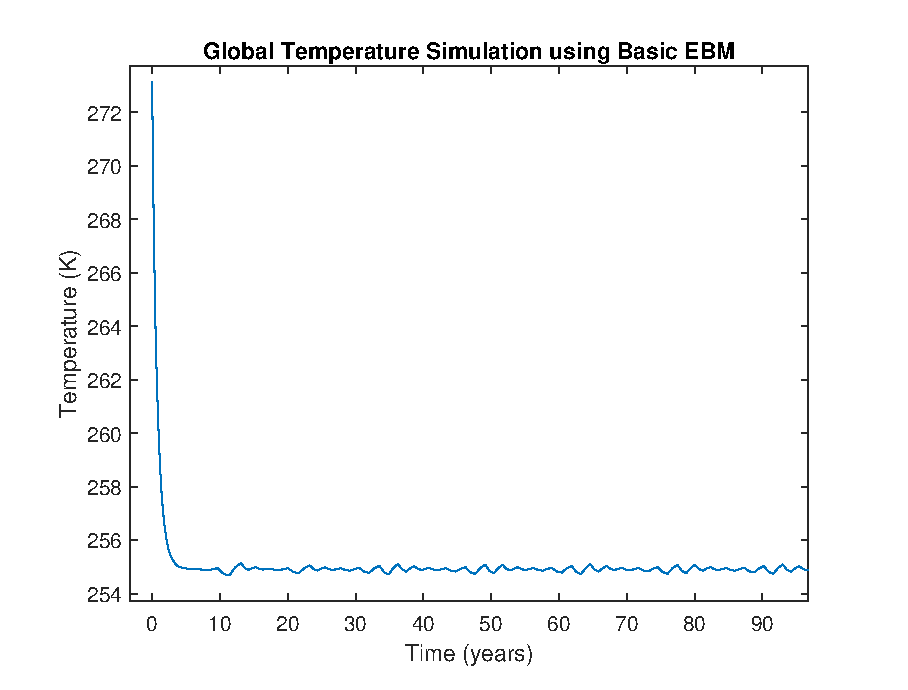
\includegraphics[width=0.8\textwidth]{images/ebm_basic.eps}
    \caption{Simulation of the basic EBM}
    \label{fig:basic_ebm}
\end{figure}

% FIXME: Do we need to repeat the values ??
% \begin{itemize}
%     \item $Q$ is the average global solar radiation (342 W/m$^2$).
%     \item $\alpha$ is the albedo of the planet (0.3).
%     \item $\sigma$ is the Stefan-Boltzmann constant ($5.67 \times 10^{-8}$ W/m$^2$/K$^4$).
%     \item $T_{eq}$ is the equilibrium temperature in Kelvin.
% \end{itemize}

\subsubsection{Albedo variation}

% FIXME: This parapgrah is very long and kind of contains an explanation on how albedo influences the earth temperature

The albedo of the Earth is not constant, and varies with the seasons. The albedo is higher in the winter due to the presence of snow and ice, and lower in the summer due to the presence of vegetation\cite{kaper-2013-math-ac-albedo}.

For an albedo ($\alpha$) of 0 (absorbing all incoming solar radiation), the equilibrium temperature is approximately 278.68 Kelvin. For an albedo of 1 (reflecting all incoming solar radiation), the equilibrium temperature is 0 Kelvin. These results highlight the significant impact of albedo on the Earth's temperature. An albedo of 1 is an extreme and theoretical scenario where all incoming solar radiation is reflected, leading to no energy absorption and hence a theoretical equilibrium temperature of absolute zero. In contrast, an albedo of 0 leads to higher temperatures due to the absorption of all incoming solar radiation.

\begin{figure}[!hbt]
    \centering
    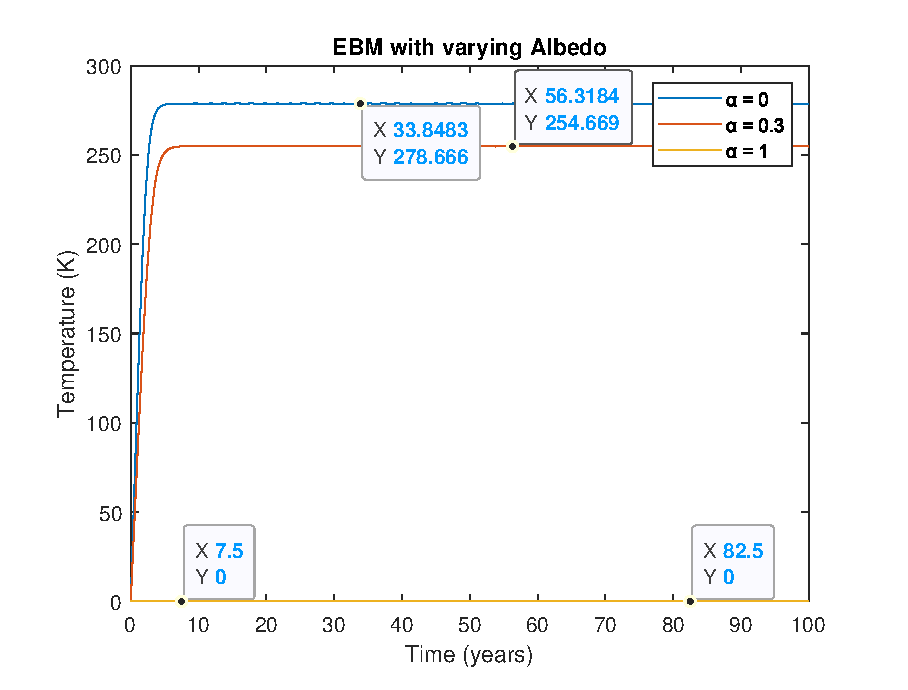
\includegraphics[width=0.8\textwidth]{images/albedo_extremes.eps}
    \caption{Simulation of the basic EBM with different albedos}
    \label{fig:albedo_extremes}
\end{figure}

\subsection{Emissivity Dependent OLR}
The equilibrium temperature of the system, considering emissivity in the Energy Balance Model (EBM), is calculated by modifying the original equation\ref{eq:equilibrium-0} to include the emissivity factor\cite{kaper-2013-math-ac-emissivity}.

\begin{equation} \label{eq:emissivity-0}
    Q(1 - \alpha) = \epsilon\sigma T^4
\end{equation}

\noindent The equation \ref{eq:emissivity-0} can then be rearranged to isolate $T$:
\begin{equation} \label{eq:emissivity-1}
    T = \left( \frac{Q(1 - \alpha)}{\epsilon\sigma} \right)^{\frac{1}{4}}
\end{equation}

\noindent The values can then be substituted in \ref{eq:emissivity-1}, which give us:
\begin{equation}
    T = \left( \frac{342 \times (1 - 0.3)}{0.61 \times 5.67 \times 10^{-8}} \right)^{\frac{1}{4}} \approx 288.44 \, \text{K} \, ({15.29}^\circ C)
\end{equation}

% FIXME: Do we need to repeat the values ??
% \begin{itemize}
%     \item $Q = 342 \, \text{W/m}^2$ (Average global solar radiation).
%     \item $\alpha = 0.3$ (Albedo).
%     \item $\sigma = 5.67 \times 10^{-8} \, \text{W/m}^2/\text{K}^4$ (Stefan-Boltzmann constant).
%     \item $\epsilon = 0.61$ (Emissivity, a typical value for Earth).
% \end{itemize}

This equilibrium temperature is much closer to the actual average surface temperature of the Earth, demonstrating the significant impact of emissivity
in the energy balance model. In the case where the Earth does not emit any longwave radiation ($\epsilon=0$), we have noticed a increase of nearly 85 Kelvin per year.

\begin{figure}[H]
    \centering
    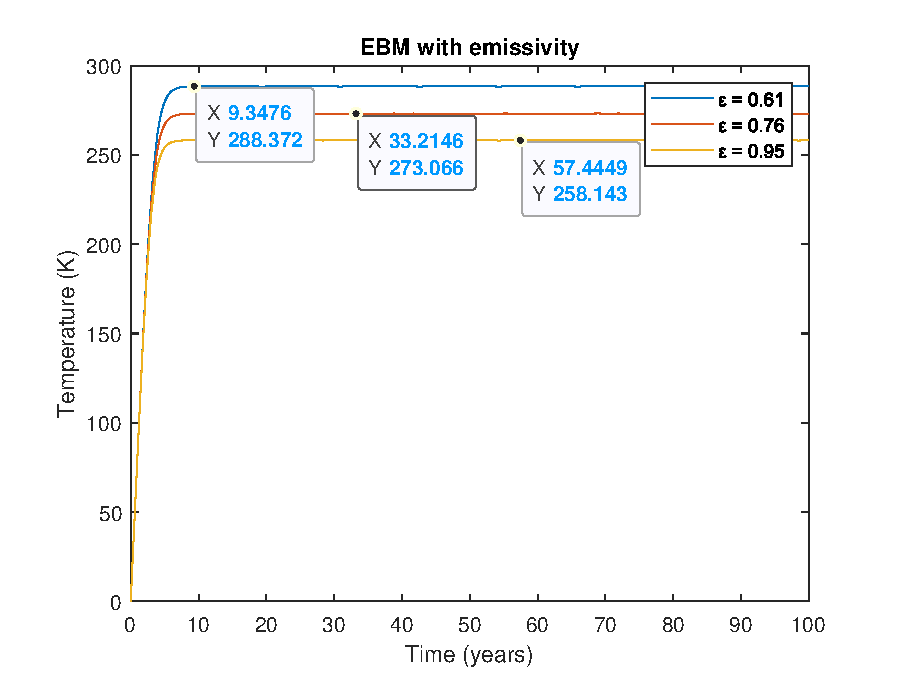
\includegraphics[width=0.8\textwidth]{images/ebm_emissivity_diff.eps}
    % \caption{Simulation of EBM with different emissivity factors}
    \caption{EBM simulation with typical $\epsilon=0.61$, $\epsilon=0.76$, showing negligible temperature change, and near maximum $\epsilon=0.95$, showing a small temperature decrease. This plot represents a more realistic scenario with a higher emissivity, resulting in minimal temperature variation over time.}

    \label{fig:ebm_emissivity}
\end{figure}

\subsection{Temperature Dependent OLR}
In this model, the Outgoing Longwave Radiation (OLR) is considered to be a function of temperature, represented by \( A + BT \), where \( A \) and \( B \) are constants. This approach acknowledges the fact that the Earth's radiation into space varies with its surface temperature\cite{kaper-2013-math-ac-budyko}.

% FIXME: Where does this comes from
The equilibrium temperature under this model, represented by the equation \( R\frac{dT}{dt} = Q(1 - \alpha) - (A + BT) \), aligns more closely with empirical observations when compared to the basic EBM. This model also accounts for feedback mechanisms that are temperature-dependent offering a more nuanced understanding of the Earth's climate system.

\begin{figure}[H]
    \centering
    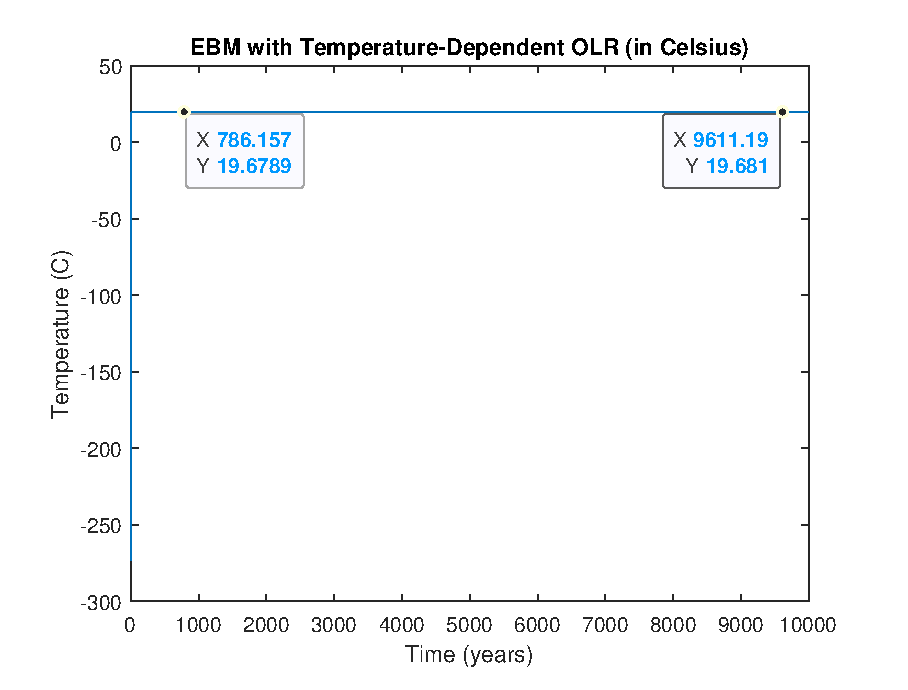
\includegraphics[width=0.8\textwidth]{images/temperature_dependent_olr.eps}
    \caption{Simulation of the EBM with temperature dependent OLR}
    \label{fig:ebm_temperature_olr}
\end{figure}

\subsection{Temperature Dependent Albedo}
The model incorporating temperature-dependent albedo reflects the dynamic nature of the Earth's surface. As the temperature varies, so does the albedo,
due to factors like melting ice and snow cover\cite{kaper-2013-math-ac-albedo}. This is represented by the equation \( \alpha(T) = 0.5 + 0.2 \tanh(0.1(265 - T - 273.5)) \).

This model introduces a feedback mechanism where rising temperatures can lead to decreased albedo, further accelerating warming—a phenomenon observed in the melting of polar ice caps.

\begin{figure}[H]
    \centering
    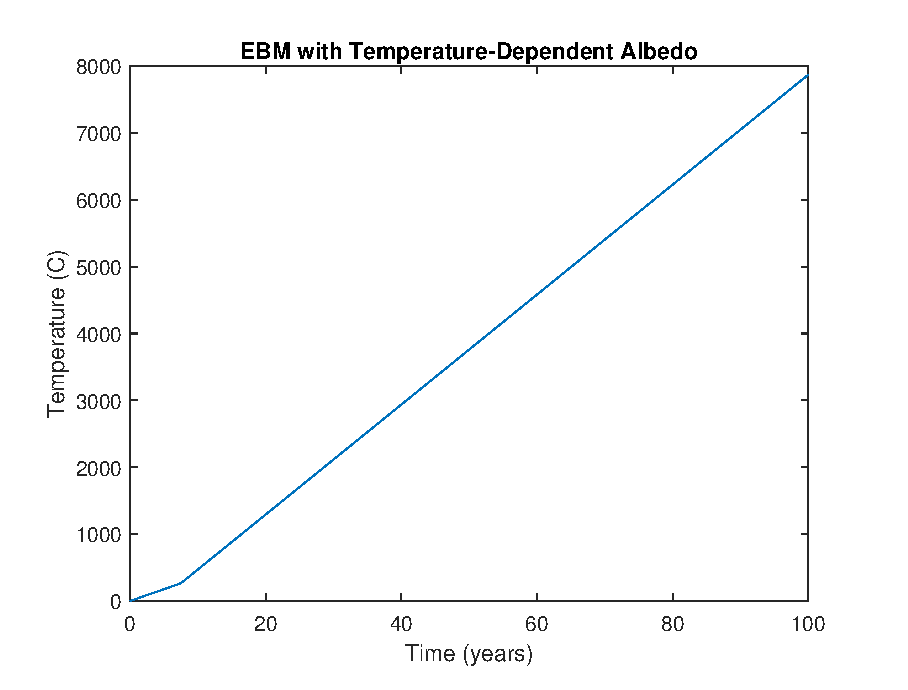
\includegraphics[width=0.8\textwidth]{images/temperature_dependent_albedo.eps}
    \label{fig:ebm_temperature_albedo}
    \caption{Simulation of the EBM with temperature-dependent albedo}
\end{figure}


\section{Discussion}
% Analyze the results you've presented.
% How do the models compare with each other?
% Discuss the implications of your findings, especially in the context of climate change.
% Are there any limitations or notable aspects of the models that affected the results?

\subsection{Analysis of Emissivity and Temperature-Dependent OLR Models}


The results from the simulations raise interesting points of discussion,
particularly regarding the relative accuracy of the models
in predicting Earth's average temperature.
The model incorporating emissivity (Question 3) yielded
a temperature closer to the real-world average of 14.84°C,
whereas the temperature-dependent OLR model (Question 4)
deviated more significantly from this value.

\subsubsection{Impact of Emissivity in Climate Models}
The inclusion of emissivity in the energy balance model significantly
enhances its realism. Emissivity, representing the Earth's ability to emit
 radiation, is a key factor in the Earth's energy balance.
 Our simulation using an emissivity factor close to Earth's real value
 (approximately 0.61) resulted in a temperature estimation that aligns
  more closely with the actual average global temperature.
  This underscores the importance of emissivity in modeling Earth's climate
  and suggests that it captures essential aspects of the Earth's radiation
   dynamics.

\subsubsection{Challenges with Temperature-Dependent OLR}
The model with temperature-dependent OLR, despite adding complexity,
may not have been as effective in mimicking the actual climate system.
The parameters \( A \) and \( B \) in the \( A + BT \) formulation of OLR
are crucial. If these parameters do not accurately reflect the Earth's real
radiation properties,
the model's predictions can deviate from real-world temperatures.
This indicates the challenge of accurately calibrating climate models
to match the complexities of the Earth's climate system.

\subsection{Model Limitations and Realism}
Both models are simplified representations of the actual climate system.
The differences in their predictions highlight the impact of various
climatic factors on Earth's temperature. It also emphasizes the need
for precise parameter selection and calibration in climate modeling.
The closer alignment of the emissivity model with the actual
average temperature suggests that, for our models,
the emissivity factor is more crucial in capturing the key aspects of
Earth's thermal radiation balance compared to the linear relationship of
temperature-dependent OLR.


\section{Conclusion}
% Summarize your main findings.
% Reflect on what these results mean for our understanding of Earth's climate system.
The comparison between the two models demonstrates
the nuanced nature of climate modeling.
It highlights the importance of choosing and
calibrating model parameters accurately to reflect
the complexities of the real-world climate system.

\bibliographystyle{unsrt}
\bibliography{bibliography}

\end{document}
